\chapter{Probability}

\begin{ex}
  Consider $B_i$ and $B_j$ with $i<j$. Suppose $x\in B_i$ and note that then
  $x\not\in B_j$, since by definition
  \[
    B_j
    =\left\{\omega\in\Omega\mid
    \omega\in A_j,\omega\not\in A_{j-1},\ldots,
    \omega\not\in A_{i}\ldots,\omega\not\in A_{1}\right\}.
  \]
  Therefore, $B_i\cap B_j=\emptyset$.

  Since the sequence of $A_i$'s is monotone increasing, it is clear that
  $A_n=\bigcup_{i=1}^n A_i$, since $A_i\subset A_n$ for all $i\leq n$. Note that
  $\bigcup_{i=1}^n B_i\subset A_n$, since $B_i\subset A_i$
  by definition. If $x\in \bigcup_{i=1}^n A_i$, then there exists a $j$ such
  that $x\in A_j$, but $x\not\in A_i$ for any $i<j$, and therefore $x\in B_j$.
  Hence, $\bigcup_{i=1}^n A_i\subset\bigcup_{i=1}^n B_i$.

  Thus, $\bigcup_{i=1}^n A_i=\bigcup_{i=1}^n B_i$ for all $n$, and therefore
  $\bigcup_{i=1}^\infty A_i=\bigcup_{i=1}^\infty B_i$. This completes the proof
  of the monotone increasing case of Theorem 1.8.

  If $A_1\supset A_2\supset\cdots$ is monotone decreasing, it follows that
  $A_1^c\subset A_2^c\subset\cdots$ is monotone increasing. Therefore,
  \[
    \lim_{n\to\infty}\P{A_n}
    =1-\lim_{n\to\infty}\P{A_n^c}
    =1-\P{A^c}
    =\P{A}.
  \]
\end{ex}

\begin{ex}
  Note that since $\emptyset\cap\emptyset=\emptyset$, the empty set is disjoint
  to itself. Therefore,
  \[
    \P{\emptyset}
    =\P{\bigsqcup_{i=1}^\infty \emptyset}
    =\sum_{i=1}^\infty\P{\emptyset}
  \]
  by Axiom 3. However, this series only converges if $\P{\emptyset}=0$.

  Suppose $A\cap B=\emptyset$. Let $C_1=A$, $C_2=B$ and $C_n=\emptyset$ for
  $n\geq 3$, and note that then $\bigcup_{i=1}^\infty C_i$ is a disjoint
  partition of $A\cup B$. Therefore,
  \[
    \P{A\cup B}
    =\P{\bigsqcup_{i=1}^\infty C_i}
    =\sum_{i=1}^\infty \P{C_i}
    =\P{A}+\P{B}+\sum_{i=3}^\infty 0
    =\P{A}+\P{B}.
  \]

  If $A\subset B$, then $B=A\sqcup (B\setminus A)$, and so by the preceding
  result,
  \[
    \P{B}=\P{A\sqcup (B\setminus A)}=\P{A}+\P{B\setminus A}.
  \]
  Therefore, since $\P{B\setminus A}\geq 0$ by Axiom 1, we get
  $\P{A}\leq \P{B}$.

  Note that $0\leq \P{A}$ is just a restatement of Axiom 1. $\P{A}\leq 1$
  follows by the previous result after observing that $A\subset \Omega$ and
  $\P{\Omega}=1$ by Axiom 2.

  Finally, note that $\Omega=A\sqcup A^c$, and therefore
  \[
    1=\P{\Omega}=\P{A}+\P{A^c}.
  \]
  Hence, $\P{A^c}=1-\P{A}$.
\end{ex}

\begin{ex}
  \begin{enumerate}[(a)]
    \item Let $s,t\in\Z_{>0}$ such that $s<t$ and note that then
          \[
            B_s
            =\bigcup_{i=s}^n A_i
            =\bigcup_{i=s}^{t-1} A_i \cup \bigcup_{i=t}^\infty A_i
            =\bigcup_{i=s}^{t-1} A_i\cup B_t.
          \]
          Therefore, $B_t \subset B_s$.

          Now consider
          \[
            C_s
            =\bigcap_{i=s}^n A_i
            =\bigcap_{i=s}^{t-1} A_i \cap \bigcap_{i=t}^\infty A_i
            =\bigcap_{i=s}^{t-1} A_i\cap C_t.
          \]
          Therefore, $C_s\subset C_t$.

    \item Suppose $\omega\in \bigcap_{n=1}^\infty B_n$. Then $\omega\in B_n$ for
          all $n$, and therefore for any $M>0$, we can find an $m>M$ such that
          $\omega\in A_m$. Hence, letting $M_1=1$, $m_i$ be the smallest integer
          greater than $M_i$ such that $\omega\in A_{m_i}$, and $M_i=m_{i-1}$
          for $i>1$, we get an infinite family of events $\{A_{m_i}\}$ such that
          $\omega\in A_{m_i}$ for all $i$.

          Conversely, suppose that $\omega\in A_n$ for infinitely many $n$. Then
          for any $B_n$, since there are only finitely many $A_i$'s with
          $i\leq n$, there must exist some $m>n$ such that $\omega\in A_m$.
          Hence, $\omega\in B_n$, and since $n$ was arbitrary,
          $\omega\in \bigcap_{n=1}^\infty B_n$.

    \item Suppose $\omega\in \bigcup_{n=1}^\infty C_n$. Then there exists some
          $m$ such that $\omega\in C_m$ and therefore
          $\omega\in\bigcap_{i=m}^\infty A_i$. Hence, $\omega\in A_i$ for all
          $i\geq m$, and thus $\omega$ belongs to all $A_i$'s except possibly
          finitely many.

          Conversely, suppose that $\omega$ belongs to all the events except
          possibly finitely many. Let $m-1$ be the largest integer such
          $\omega\not\in A_{m-1}$ and note that then
          $\omega\in \bigcap_{i=m}^\infty A_i=C_m$. Hence,
          $\omega\in \bigcup_{n=1}^\infty C_n$.
  \end{enumerate}
\end{ex}

\begin{ex}
  Suppose $x\in\bigcap_{i\in I}A_i^c$. Then for all $i\in I$, $x\in A_i^c$ and
  therefore $x\not\in A_i$ for all $i\in I$. Hence,
  $x\not\in \bigcup_{i\in I} A_i$ and $x\in\left(\bigcup_{i\in I} A_i\right)^c$.
  Thus, $\bigcap_{i\in I}A_i^c\subset \left(\bigcup_{i\in I} A_i\right)^c$.

  Suppose $x\in\left(\bigcup_{i\in I} A_i\right)^c$. Then
  $x\not\in\bigcup_{i\in I} A_i$, and hence $x\not\in A_i$ for all $i\in I$.
  Thus, $x\in A_i^c$ for all $i\in I$ and so $x\in\bigcap_{i\in I}A_i^c$. Hence,
  $\left(\bigcup_{i\in I} A_i\right)^c\subset\bigcap_{i\in I}A_i^c$, and
  therefore
  \[
    \left(\bigcup_{i\in I} A_i\right)^c=\bigcap_{i\in I}A_i^c.
  \]

  Replacing $A_i$ with $A_i^c$, taking the complement of both sides and using
  the fact that the complement of a complement is the original set, it follows
  that
  \[
    \bigcup_{i\in I} A_i^c=\left(\bigcap_{i\in I}A_i\right)^c.
  \]
\end{ex}

\begin{ex}
  The sample space is
  \[
    S=\left\{
    \underbrace{T\cdots T}_{n_1\text{ times}}
    H\underbrace{T\cdots T}_{n_2\text{ times}}H \mid n_1,n_2\geq0 \right\}.
  \]
  Note that if exactly $k$ tosses are required, the final coin toss is always
  the second heads, but the first heads can occur on any of the preceding $k-1$
  tosses. Hence, for $k\geq 2$ the probability of this event is
  \[
    (k-1)\left(\frac{1}{2}\right)^k.
  \]
\end{ex}

\begin{ex}
  Suppose that there exists such a distribution. Let $p=\P{\{0\}}$ and note that
  $p\neq 0$, since otherwise $1=\P{\Omega}=\sum_{i=0}^n\P{\{i\}}=0$, a
  contradiction. Therefore, we can let
  $N=\left\lceil\frac{1}{p}\right\rceil+1$ and $A=\{0, 1, \ldots, N-1\}$. Then
  \begin{align*}
    \P{A}
    =N\P{\{0\}}
    =\left(\left\lceil\frac{1}{p}\right\rceil+1\right)p
    \geq 1 + p,
  \end{align*}
  contradicting the requirement that probability is between $0$ and $1$.
  Therefore, no such distribution can exist.
\end{ex}

\begin{ex}
  Let $B_n=A_n\setminus \bigcup_{i=1}^{n-1}A_i$. Consider $B_s$ and $B_t$ such
  that $s<t$ and note that if $x$ is an element of $B_s$, by definition $x$ must
  be an element of $A_s$. Hence, since $t>s$,
  $x\in\bigcup_{i=1}^{t-1} A_i$, and thus
  $x\not\in A_t\setminus \bigcup_{i=1}^{t-1}A_i=B_t$. Therefore, $B_s$ and $B_t$
  are disjoint whenever $s\neq t$.

  Since $B_n\subset A_n$ for all $n$, it follows that
  $\bigcup_{n=1}^\infty B_n\subset \bigcup_{n=1}^\infty A_n$. Moreover, if
  $x\in \bigcup_{n=1}^\infty A_n$ there exists some $m$ such that $x\in A_m$,
  but $x\not\in A_s$, for $s<m$. This implies that $x\in B_m$ and therefore
  $\bigcup_{n=1}^\infty A_n\subset \bigcup_{n=1}^\infty B_n$. Hence,
  $\bigcup_{n=1}^\infty A_n= \bigcup_{n=1}^\infty B_n$.

  Thus,
  \[
    \P{\bigcup_{n=1}^\infty A_n}
    =\P{\bigsqcup_{n=1}^\infty B_n}
    =\sum_{n=1}^\infty \P{B_n}
    \leq \sum_{n=1}^\infty \P{A_n},
  \]
  since $B_n\subset A_n$ for all $n$.
\end{ex}

\begin{ex}
  \begin{align*}
    \P{\bigcap_{i=1}^\infty A_i}
     & =1-\P{\bigcup_{i=1}^\infty A_i^c} &  & \text{(by De Morgan's law)}  \\
     & \geq 1-\sum_{i=1}^\infty\P{A_i^c} &  & \text{(by previous problem)} \\
     & =1.
  \end{align*}
\end{ex}

\begin{ex}
  Note that for any event $A$, we have
  \[
    \cP{A}{B}
    =\frac{\P{A\cap B}}{\P{B}}\geq 0,
  \]
  since $\P{B}> 0$ and $\P{A\cap B}\geq 0$ by the first axiom of probability,
  and therefore $\cP{\,\cdot}{B}$ also satisfies the first axiom.

  We also have
  \[
    \cP{\Omega}{B}=\frac{\P{\Omega\cap B}}{\P{B}}=\frac{\P{B}}{\P{B}}=1,
  \]
  and therefore $\cP{\,\cdot\,}{B}$ satisfies the second axiom.

  Finally, suppose that $A_1, A_2, \ldots$ are disjoint. Then
  \begin{align*}
    \cP{\bigcup_{i=1}^\infty A_i}{B}
     & =\frac{\P{\bigcup_{i=1}^\infty A_i\cap B}}{\P{B}} \\
     & =\frac{1}{\P{B}}\sum_{i=1}^\infty \P{A_i \cap B}  \\
     & =\sum_{i=1}^\infty \frac{\P{A_i \cap B}}{\P{B}}   \\
     & =\sum_{i=1}^\infty \cP{A_i}{B},
  \end{align*}
  and therefore $\cP{\,\cdot}{B}$ satisfies the third axiom.
\end{ex}

\begin{ex}
  Without loss of generality, we may assume that the player initially selects
  the first door and the host reveals the second door to be empty. Then, letting
  $D_i$ be the event of the reward being behind door $i$ and $R_2$ being the
  event of the host opening door $2$, we have
  \begin{align*}
    \cP{D_1}{R_2}
    =\frac{\cP{R_2}{D_1}\P{D_1}}{\P{R_2}}
    =\frac{\frac{1}{2}\cdot\frac{1}{3}}{\frac{1}{2}}=\frac{1}{3},
  \end{align*}
  for Door 1 and
  \begin{align*}
    \cP{D_3}{R_2}
    =\frac{\cP{R_2}{D_3}\P{D_3}}{\P{R_2}}
    =\frac{1\cdot\frac{1}{3}}{\frac{1}{2}}=\frac{2}{3},
  \end{align*}
  for Door 3, since if the reward were behind Door 1 the host would have been
  able to reveal either Door 2 or Door 3, but if it were behind Door 3, he
  would be forced to reveal Door 2.
\end{ex}

\begin{ex}
  \begin{align*}
    \P{A^c\cap B^c}
     & =\P{(A^{c^c}\cup B^{c^c})^c}                  &  & \text{(by De Morgan's law)} \\
     & =\P{(A \cup B)^c}                                                              \\
     & =1 - \P{A\cup B}                                                               \\
     & =1 - \left[\P{A} + \P{B} - \P{A\cap B}\right]                                  \\
     & =1-\P{A}-\P{B}+\P{A}\P{B}                     &  & \text{(since $A\amalg B$)}  \\
     & =\left[1-\P{A}\right]\left[1-\P{B}\right]                                      \\
     & =\P{A^c}\P{B^c}
  \end{align*}
\end{ex}

\begin{ex}
  Let $S_g$ be the event of drawing a card showing a green side and $C_g$ be the
  event of drawing the card that is green on both sides. Then, by Bayes'
  theorem,
  \begin{align*}
    \cP{C_g}{S_g}
     & =\frac{\cP{S_g}{C_g}\P{C_g}}{\P{S_g}}
    =\frac{1\cdot \frac{1}{3}}{\frac{1}{2}}
    =\frac{2}{3}.
  \end{align*}
\end{ex}

\begin{ex}
  \begin{enumerate}[(a)]
    \item The sample space is given by
          \[
            S=\left\{
            \underbrace{T\cdots T}_{n\text{ times}}H \mid n\geq 1
            \right\} \bigcup
            \left\{
            \underbrace{H\cdots H}_{n\text{ times}}T \mid n\geq 1
            \right\}.
          \]
    \item There are two possible ways that can happen: by throwing $HHT$ or
          $TTH$. Therefore, the probability is
          \[
            2\cdot \left(\frac{1}{2}\right)^3=\frac{1}{4}.
          \]
  \end{enumerate}
\end{ex}

\begin{ex}
  Let $\P{A}=0$ and let $B$ be an arbitrary event. Then it is clear that
  \[
    0\leq \P{A\cap B}\leq \P{A}=0,
  \]
  and therefore $\P{A\cap B}=\P{A}\P{B}$ trivially. Hence, $A\amalg B$.

  Otherwise, if $\P{A}=1$, note that $\P{A^c}=0$, and therefore $A^c\amalg B^c$
  for any event $B^c$. However, Exercise 11 then implies that $A\amalg B$.

  If $A$ is independent of itself, we have $\P{A}=\P{A\cap A}=[\P{A}]^2$, and
  therefore $\P{A}$ must equal $0$ or $1$.
\end{ex}

\begin{ex}
  \begin{enumerate}[(a)]
    \item Having at least two children with blue eyes corresponds to the event
          $\{BBO, BOB, OBB,$ $BBB\}$. Note that by Bayes' theorem
          \[
            \cP{BBO}{B_{\geq 1}}
            =\frac{\cP{B_{\geq 1}}{BBO}\P{BBO}}{\P{B_{\geq 1}}}
            =\frac{1\cdot \frac{3}{64}}{\frac{37}{64}}
            =\frac{3}{37},
          \]
          and similarly $\cP{BOB}{B_{\geq 1}}=\cP{OBB}{B_{\geq 1}}=\frac{3}{37}$
          by independence between children. Meanwhile,
          \[
            \cP{BBB}{B_{\geq 1}}
            =\frac{\cP{B_{\geq 1}}{BBB}\P{BBB}}{\P{B_{\geq 1}}}
            =\frac{1\cdot \frac{1}{64}}{\frac{37}{64}}
            =\frac{1}{37}.
          \]
          Therefore, the probability at least two children have blue eyes given
          that at least one child has blue eyes is $\frac{10}{37}$.

    \item This is identical to asking what is the probability that at least one
          of the two remaining children has blue eyes. The probability that
          either the middle or eldest child, but not both, have blue eyes is
          $2\cdot \frac{1}{4}\cdot\frac{3}{4}=\frac{3}{8}$, while the
          probability that both have blue eyes is $\frac{1}{16}$. Therefore,
          the probability that at least two children have blue eyes given that
          the youngest child has blue eyes is $\frac{7}{16}$.
  \end{enumerate}
\end{ex}

\begin{ex}
  If $A$ and $B$ are independent events, then
  \[
    \cP{A}{B}=\frac{\P{A\cap B}}{\P{B}}=\frac{\P{A}\P{B}}{\P{B}}=\P{A}.
  \]

  For any events $A$ and $B$, the definition of conditional probability states
  that
  \[
    \cP{A}{B}=\frac{\P{A\cap B}}{\P{B}}\text{, and }
    \cP{B}{A}=\frac{\P{A\cap B}}{\P{A}}.
  \]
  Solving both for $\P{A\cap B}$ gives us
  \[
    \P{A\cap B}=\cP{A}{B}\P{B}=\cP{B}{A}\P{A}.
  \]
\end{ex}

\begin{ex}
  This is immediate from applying the definition of conditional probability
  twice, first to $A\,|\,B\cap C$ and then to $B\,|\,C$,
  \begin{align*}
    \P{A\cap B\cap C}
    =\cP{A}{B\cap C}\P{B\cap C}
    =\cP{A}{B\cap C}\cP{B}{C}\P{C}.
  \end{align*}
\end{ex}

\begin{ex}
  Let $\P{A_1}-\cP{A_1}{B}=\varepsilon$ and suppose that
  $\cP{A_i}{B}\leq \P{A_i}$ for all $i=2,\ldots,k$. Then
  \begin{align*}
    0 & = \sum_{i=1}^k\P{A_i}-\sum_{i=1}^k\cP{A_i}{B}                      \\
      & = \P{A_1}-\cP{A_1}{B}+\sum_{i=2}^k\left(\P{A_i}-\cP{A_i}{B}\right) \\
      & \geq \varepsilon,
  \end{align*}
  a contradiction. Therefore, $\cP{A_i}{B}> \P{A_i}$ for some $i$.
\end{ex}

\begin{ex}
  \begin{align*}
    \cP{W}{+}
     & =\frac{\cP{+}{W}\P{W}}{\P{+}}                                          &  & \text{(by Bayes' theorem)} \\
     & =\frac{0.82 \cdot 0.5}{0.65\cdot 0.3 + 0.82 \cdot 0.5 + 0.5 \cdot 0.2}                                 \\
     & =0.58.
  \end{align*}
\end{ex}

\begin{ex}
  \begin{enumerate}[(a)]
    \item Note that by Bayes' theorem,
          \[
            \cP{C_i}{H}
            =\frac{\cP{H}{C_i}\P{C_i}}{\sum_{j=1}^5 \cP{H}{C_j}\P{C_j}}
          \]
          where
          \[
            \sum_{j=1}^5 \cP{H}{C_j}\P{C_j}
            =\frac{1}{4}\cdot\frac{1}{5}+\frac{1}{2}\cdot\frac{1}{5}
            +\frac{3}{4}\cdot\frac{1}{5}+1\cdot\frac{1}{5}
            =\frac{1+2+3+4}{20}=\frac{1}{2}.
          \]

          Hence,
          \[
            \cP{C_1}{H} = 0,\,
            \cP{C_2}{H} = \frac{1}{10},\,
            \cP{C_3}{H} = \frac{1}{5},\,
            \cP{C_4}{H} = \frac{3}{10}\text{, and }
            \cP{C_5}{H} = \frac{2}{5}.
          \]
    \item
          \[
            \cP{H_2}{H_1}
            =\sum_{j=1}^5\cP{H}{C_j}\cP{C_j}{H}
            =0+\frac{1}{4}\cdot\frac{1}{10}
            +\frac{1}{2}\cdot\frac{1}{5}
            +\frac{3}{4}\cdot\frac{3}{10}
            +1\cdot\frac{2}{5}=\frac{3}{4}.
          \]
    \item Note that
          \[
            \cP{B_4}{C_1}=0,\,
            \cP{B_4}{C_2}=\frac{27}{256},\,
            \cP{B_4}{C_3}=\frac{1}{16},\,
            \cP{B_4}{C_4}=\frac{3}{256}\text{, and }
            \cP{B_4}{C_5}=0,
          \]
          and,
          \[
            \sum_{j=1}^5 \cP{B_4}{C_j}\P{C_j}
            =0+\frac{1}{5}\cdot\frac{27}{256}+\frac{1}{5}\cdot\frac{1}{16}
            +\frac{1}{5}\cdot\frac{3}{256}+0
            =\frac{23}{640}.
          \]
          Therefore, by Bayes' theorem,
          \[
            \cP{C_1}{B_4} = 0,\,
            \cP{C_2}{B_4} = \frac{27}{46},\,
            \cP{C_3}{B_4} = \frac{8}{23},\,
            \cP{C_4}{B_4} = \frac{3}{46}\text{, and }
            \cP{C_5}{B_4} = 0.
          \]
  \end{enumerate}
\end{ex}

\begin{ex}~
  \inputminted{python}{../code/01-21.py}

  \begin{figure}[H]
    \centering
    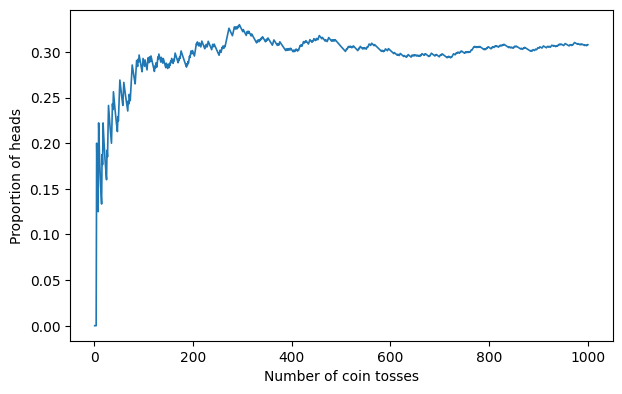
\includegraphics[scale=0.8]{../images/01-21a}
    \caption{Proportion of heads as a function of the number of coin flips for
      $p_\text{heads}=0.3$.}
  \end{figure}

  \begin{figure}[H]
    \centering
    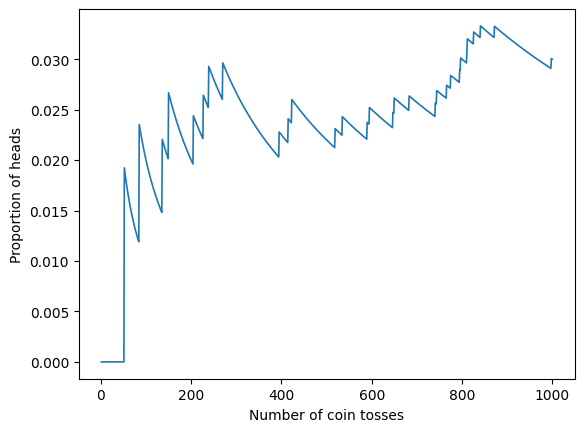
\includegraphics[scale=0.8]{../images/01-21b}
    \caption{Proportion of heads as a function of the number of coin flips for
      $p_{heads}=0.03$.}
  \end{figure}

\end{ex}

\begin{ex}~
  \inputminted{python}{../code/01-22.py}
  \inputminted{text}{../output/01-22.txt}
\end{ex}

\begin{ex}~
  \inputminted{python}{../code/01-23.py}
  \inputminted{text}{../output/01-23.txt}

  In the case of $A=\{2, 4, 6\}$ and $B=\{1, 2, 3, 4\}$, the theoretical values
  are $\P{A}=\frac{1}{2}$, $\P{B}=\frac{2}{3}$ and $\P{AB}=\frac{1}{3}$.

  For $A=\{1, 2, 3, 4\}$ and $B=\{3, 4, 5, 6\}$, the theoretical values are
  $\P{A}=\frac{2}{3}$, $\P{B}=\frac{2}{3}$ and $\P{AB}=\frac{1}{3}$.
\end{ex}